\documentclass[border=6pt,multi=tikzpicture]{standalone}
\usepackage{tikz}
\usetikzlibrary{arrows.meta,positioning,calc,fit,backgrounds,shapes.geometric}

\definecolor{bblue}{HTML}{2A78D6}
\definecolor{borange}{HTML}{EB6834}
\definecolor{btint}{HTML}{DCE9F8}
\definecolor{bwarm}{HTML}{FDECE4}
\definecolor{bink}{HTML}{0B0B0B}
\definecolor{binkb}{HTML}{52514E}
\definecolor{bpaper}{HTML}{F4F4F2}
\definecolor{bline}{HTML}{C8C7C2}

\tikzset{
  icon/.style={line width=0.5pt, draw=#1, line cap=round, line join=round},
  pics/ic person/.style n args={1}{code={\begin{scope}[icon=#1]
      \draw (0,0.085) circle (0.055);
      \draw (-0.095,-0.095) .. controls (-0.095,0.02) and (0.095,0.02) .. (0.095,-0.095);
    \end{scope}}},
  pics/ic funnel/.style n args={1}{code={\begin{scope}[icon=#1]
      \draw (-0.125,0.10) -- (0.125,0.10) -- (0.033,-0.02) -- (0.033,-0.11)
            -- (-0.033,-0.07) -- (-0.033,-0.02) -- cycle;
    \end{scope}}},
  pics/ic store/.style n args={1}{code={\begin{scope}[icon=#1]
      \draw (-0.09,0.085) -- (-0.09,-0.085) arc (180:360:0.09 and 0.042) -- (0.09,0.085);
      \draw (0,0.085) ellipse (0.09 and 0.042);
      \draw (-0.09,0.0) arc (180:360:0.09 and 0.042);
    \end{scope}}},
  pics/ic scale/.style n args={1}{code={\begin{scope}[icon=#1]
      \draw (0,-0.115) -- (0,0.105);
      \draw (-0.135,0.07) -- (0.135,0.07);
      \draw (-0.135,0.07) -- (-0.19,-0.025) -- (-0.08,-0.025) -- cycle;
      \draw (0.135,0.07) -- (0.08,-0.025) -- (0.19,-0.025) -- cycle;
      \draw (-0.07,-0.115) -- (0.07,-0.115);
    \end{scope}}},
  pics/ic check/.style n args={1}{code={\begin{scope}[icon=#1,line width=0.8pt]
      \draw (-0.11,0.0) -- (-0.03,-0.08) -- (0.12,0.09);
    \end{scope}}},
  pics/ic half/.style n args={1}{code={\begin{scope}[icon=#1]
      \draw (0,0) circle (0.10);
      \fill[#1] (0,0) -- (0.10,0) arc (0:180:0.10) -- cycle;
    \end{scope}}},
  pics/ic warn/.style n args={1}{code={\begin{scope}[icon=#1]
      \draw[rounded corners=0.6pt] (0,0.12) -- (0.13,-0.10) -- (-0.13,-0.10) -- cycle;
      \draw (0,0.05) -- (0,-0.02);
      \fill[#1] (0,-0.058) circle (0.013);
    \end{scope}}},
  pics/ic link/.style n args={1}{code={\begin{scope}[icon=#1]
      \draw[rounded corners=1.1pt] (-0.14,-0.042) rectangle (0.012,0.052);
      \draw[rounded corners=1.1pt] (-0.012,-0.052) rectangle (0.14,0.042);
    \end{scope}}},
  pics/ic doc/.style n args={1}{code={\begin{scope}[icon=#1]
      \draw (-0.08,-0.11) -- (-0.08,0.11) -- (0.03,0.11) -- (0.08,0.058)
            -- (0.08,-0.11) -- cycle;
      \draw (0.03,0.11) -- (0.03,0.058) -- (0.08,0.058);
      \draw (-0.045,0.018) -- (0.045,0.018);
      \draw (-0.045,-0.04) -- (0.045,-0.04);
    \end{scope}}},
  pics/ic probe/.style n args={1}{code={\begin{scope}[icon=#1]
      \draw (-0.02,0.028) circle (0.072);
      \draw (0.032,-0.024) -- (0.11,-0.10);
    \end{scope}}},
  pics/ic tree/.style n args={1}{code={\begin{scope}[icon=#1]
      \draw (0,0.085) -- (0,0.02); \draw (-0.115,0.02) -- (0.115,0.02);
      \draw (-0.115,0.02) -- (-0.115,-0.035); \draw (0.115,0.02) -- (0.115,-0.035);
      \fill[#1] (0,0.115) circle (0.030);
      \fill[#1] (-0.115,-0.065) circle (0.030);
      \fill[#1] (0.115,-0.065) circle (0.030);
    \end{scope}}},
  pics/ic shield/.style n args={1}{code={\begin{scope}[icon=#1]
      \draw (0,0.115) -- (0.10,0.07) -- (0.10,-0.03)
            .. controls (0.10,-0.085) and (0.05,-0.10) .. (0,-0.125)
            .. controls (-0.05,-0.10) and (-0.10,-0.085) .. (-0.10,-0.03)
            -- (-0.10,0.07) -- cycle;
    \end{scope}}},
}

\newcommand{\ico}[2]{\tikz[baseline=-0.62ex]{\pic{ic #1={#2}};}}

\tikzset{
  bx/.style={draw=bink, fill=white, rounded corners=1.6pt, line width=0.45pt,
             align=center, font=\scriptsize, inner sep=2.8pt,
             execute at begin node={\hyphenpenalty=10000\exhyphenpenalty=10000}},
  bxhi/.style={bx, draw=bblue, fill=btint, line width=0.75pt},
  bxwarn/.style={bx, draw=borange, fill=bwarm, line width=0.75pt},
  bxsoft/.style={bx, fill=bpaper, draw=binkb, line width=0.4pt},
  flow/.style={-{Latex[length=3.6pt,width=2.8pt]}, draw=bink, line width=0.5pt},
  faint/.style={-{Latex[length=3pt,width=2.4pt]}, draw=binkb, line width=0.35pt},
  escal/.style={-{Latex[length=3.2pt,width=2.6pt]}, draw=borange, line width=0.5pt,
              dash pattern=on 1.7pt off 1.3pt},
  band/.style={rounded corners=2.5pt, draw=bline, line width=0.5pt, fill=white},
  bandlab/.style={font=\scriptsize\itshape, text=binkb, inner sep=1.5pt},
  capt/.style={font=\scriptsize\itshape, text=binkb, align=center},
}

\begin{document}

% =========================================================== FIGURE 1 ======
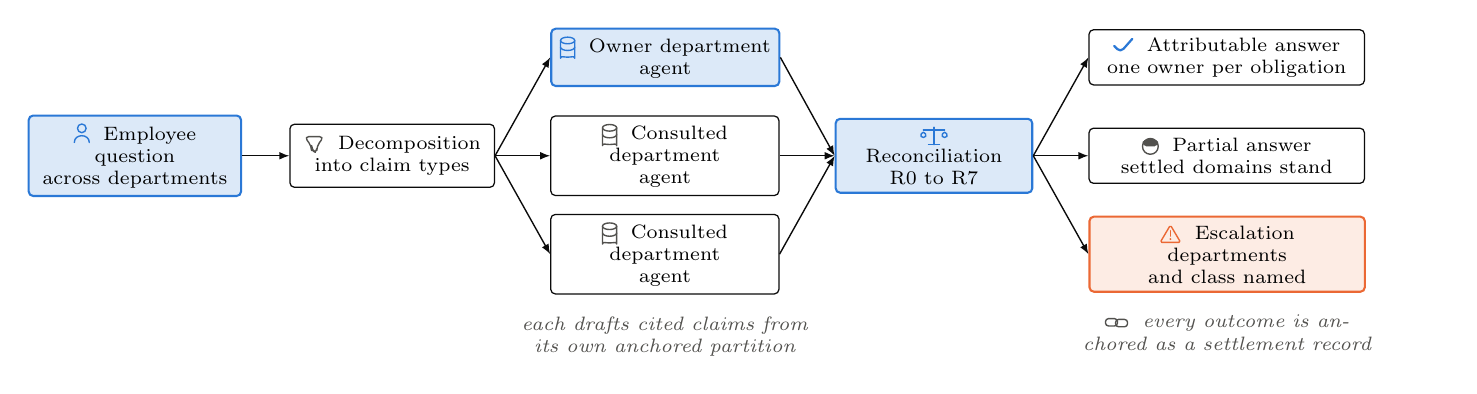
\begin{tikzpicture}
  \node[bxhi, text width=25mm, minimum height=8mm] (q)
    {\ico{person}{bblue}\; Employee question\\ across departments};
  \node[bx, right=6mm of q, text width=24mm, minimum height=8mm] (dec)
    {\ico{funnel}{binkb}\; Decomposition\\ into claim types};

  \node[bxhi, right=7mm of dec, text width=27mm, minimum height=7mm, yshift=12.5mm] (own)
    {\ico{store}{bblue}\; Owner department\\ agent};
  \node[bx, right=7mm of dec, text width=27mm, minimum height=7mm] (c1)
    {\ico{store}{binkb}\; Consulted department\\ agent};
  \node[bx, right=7mm of dec, text width=27mm, minimum height=7mm, yshift=-12.5mm] (c2)
    {\ico{store}{binkb}\; Consulted department\\ agent};

  \node[bxhi, right=7mm of c1, text width=23mm, minimum height=8mm] (rec)
    {\ico{scale}{bblue}\; Reconciliation\\ R0 to R7};

  \node[bx, right=7mm of rec, text width=33mm, minimum height=7mm, yshift=12.5mm] (o1)
    {\ico{check}{bblue}\; Attributable answer\\ one owner per obligation};
  \node[bx, right=7mm of rec, text width=33mm, minimum height=7mm] (o2)
    {\ico{half}{binkb}\; Partial answer\\ settled domains stand};
  \node[bxwarn, right=7mm of rec, text width=33mm, minimum height=7mm, yshift=-12.5mm] (o3)
    {\ico{warn}{borange}\; Escalation\\ departments and class named};

  \draw[flow] (q) -- (dec);
  \foreach \t in {own,c1,c2} \draw[flow] (dec.east) -- (\t.west);
  \foreach \s in {own,c1,c2} \draw[flow] (\s.east) -- (rec.west);
  \foreach \t in {o1,o2,o3} \draw[flow] (rec.east) -- (\t.west);

  \node[capt, below=1.6mm of c2, text width=40mm]
    {each drafts cited claims from its own anchored partition};

  \node[capt, below=1.6mm of o3, text width=54mm]
    {\ico{link}{binkb}\; every outcome is anchored as a settlement record};
\end{tikzpicture}

% =========================================================== FIGURE 2 ======
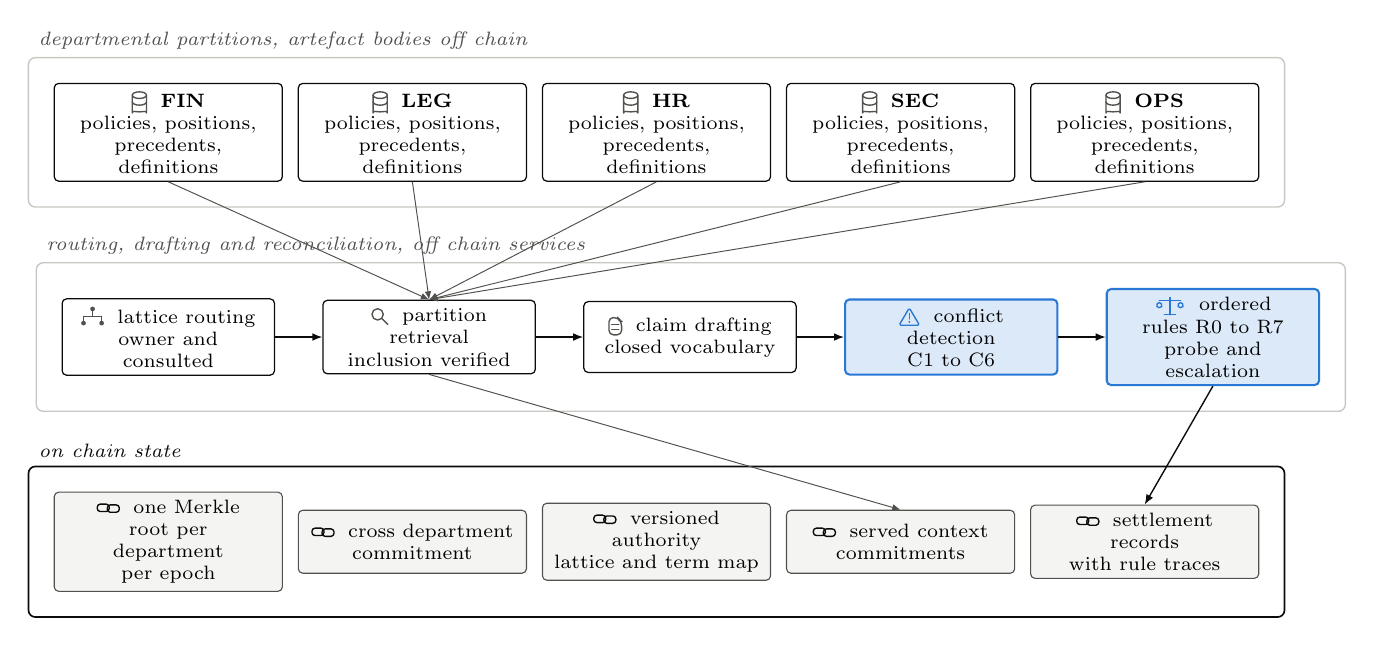
\begin{tikzpicture}[every node/.style={font=\scriptsize}]
  % band 1: partitions
  \foreach \d/\i in {FIN/0, LEG/1, HR/2, SEC/3, OPS/4} {
    \node[bx, text width=27mm, minimum height=9mm] (p\i) at (\i*31mm, 0)
      {\ico{store}{binkb}\; \textbf{\d}\\ policies, positions,\\ precedents, definitions};
  }
  \begin{scope}[on background layer]
    \node[band, fit=(p0)(p4), inner sep=3.2mm] (band1) {};
  \end{scope}
  \node[bandlab, anchor=south west] at ($(band1.north west)+(0.8mm,0.4mm)$)
    {departmental partitions, artefact bodies off chain};

  % band 2: services
  \node[bx, text width=25mm, minimum height=9mm] (s0) at (0,-26mm)
    {\ico{tree}{binkb}\; lattice routing\\ owner and consulted};
  \node[bx, right=6mm of s0, text width=25mm, minimum height=9mm] (s1)
    {\ico{probe}{binkb}\; partition retrieval\\ inclusion verified};
  \node[bx, right=6mm of s1, text width=25mm, minimum height=9mm] (s2)
    {\ico{doc}{binkb}\; claim drafting\\ closed vocabulary};
  \node[bxhi, right=6mm of s2, text width=25mm, minimum height=9mm] (s3)
    {\ico{warn}{bblue}\; conflict detection\\ C1 to C6};
  \node[bxhi, right=6mm of s3, text width=25mm, minimum height=9mm] (s4)
    {\ico{scale}{bblue}\; ordered rules R0 to R7\\ probe and escalation};
  \begin{scope}[on background layer]
    \node[band, fit=(s0)(s4), inner sep=3.2mm] (band2) {};
  \end{scope}
  \node[bandlab, anchor=south west] at ($(band2.north west)+(0.8mm,0.4mm)$)
    {routing, drafting and reconciliation, off chain services};

  \foreach \a/\b in {s0/s1, s1/s2, s2/s3, s3/s4} \draw[flow] (\a) -- (\b);
  \foreach \i in {0,1,2,3,4} \draw[faint] (p\i.south) -- ($(s1.north)+(0,0)$);

  % band 3: on chain
  \foreach \t/\i in {%
      {one Merkle root per\\ department per epoch}/0,
      {cross department\\ commitment}/1,
      {versioned authority\\ lattice and term map}/2,
      {served context\\ commitments}/3,
      {settlement records\\ with rule traces}/4} {
    \node[bxsoft, text width=27mm, minimum height=8mm] (l\i) at (\i*31mm, -52mm)
      {\ico{link}{bink}\; \t};
  }
  \begin{scope}[on background layer]
    \node[band, fit=(l0)(l4), inner sep=3.2mm, draw=bink, line width=0.6pt] (band3) {};
  \end{scope}
  \node[bandlab, anchor=south west, text=bink] at ($(band3.north west)+(0.8mm,0.4mm)$)
    {on chain state};

  \draw[faint] (s1.south) -- (l3.north);
  \draw[flow] (s4.south) -- (l4.north);
\end{tikzpicture}

% =========================================================== FIGURE 3 ======
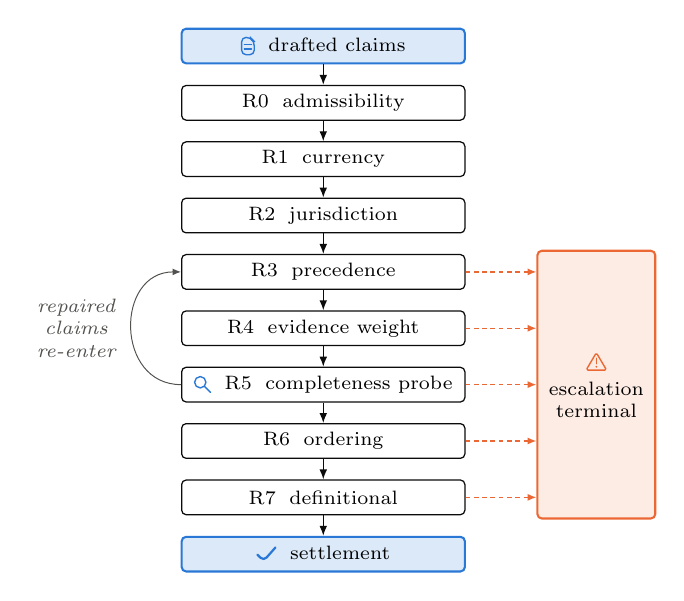
\begin{tikzpicture}[every node/.style={font=\scriptsize}]
  \def\rw{34mm}
  \node[bxhi, text width=\rw, minimum height=4.4mm] (n0) {\ico{doc}{bblue}\; drafted claims};
  \node[bx, below=2.6mm of n0, text width=\rw, minimum height=4.4mm] (n1) {R0\; admissibility};
  \node[bx, below=2.6mm of n1, text width=\rw, minimum height=4.4mm] (n2) {R1\; currency};
  \node[bx, below=2.6mm of n2, text width=\rw, minimum height=4.4mm] (n3) {R2\; jurisdiction};
  \node[bx, below=2.6mm of n3, text width=\rw, minimum height=4.4mm] (n4) {R3\; precedence};
  \node[bx, below=2.6mm of n4, text width=\rw, minimum height=4.4mm] (n5) {R4\; evidence weight};
  \node[bx, below=2.6mm of n5, text width=\rw, minimum height=4.4mm] (n6)
    {\ico{probe}{bblue}\; R5\; completeness probe};
  \node[bx, below=2.6mm of n6, text width=\rw, minimum height=4.4mm] (n7) {R6\; ordering};
  \node[bx, below=2.6mm of n7, text width=\rw, minimum height=4.4mm] (n8) {R7\; definitional};
  \node[bxhi, below=2.6mm of n8, text width=\rw, minimum height=4.4mm] (n9)
    {\ico{check}{bblue}\; settlement};

  \foreach \a/\b in {n0/n1,n1/n2,n2/n3,n3/n4,n4/n5,n5/n6,n6/n7,n7/n8,n8/n9}
    \draw[flow] (\a) -- (\b);

  \node[bxwarn, text width=13mm, minimum height=34mm, right=9mm of n6, anchor=west] (esc)
    {\ico{warn}{borange}\\[2pt] escalation\\ terminal};
  \foreach \s in {n4,n5,n6,n7,n8} \draw[escal] (\s.east) -- (esc.west |- \s);

  \draw[faint] (n6.west) to[out=180,in=180,looseness=1.5] node[left=0.8mm, midway,
      font=\scriptsize\itshape, text=binkb, align=center] {repaired\\claims\\re-enter} (n4.west);
\end{tikzpicture}

\end{document}
